\documentclass[border=10pt]{standalone}
\usepackage[utf8]{inputenc}
\usepackage[T1]{fontenc}
\usepackage{lmodern}
\usepackage{tikz}
\usetikzlibrary{arrows.meta, positioning, shapes.geometric, calc, fit}

% FehrAdvice Colors
\definecolor{fadarkblue}{RGB}{2,64,121}
\definecolor{falightblue}{RGB}{84,158,222}
\definecolor{fadarkgray}{RGB}{37,33,42}
\definecolor{falightgray}{RGB}{243,245,247}
\definecolor{famint}{RGB}{126,189,172}
\definecolor{faorange}{RGB}{222,157,62}

\begin{document}
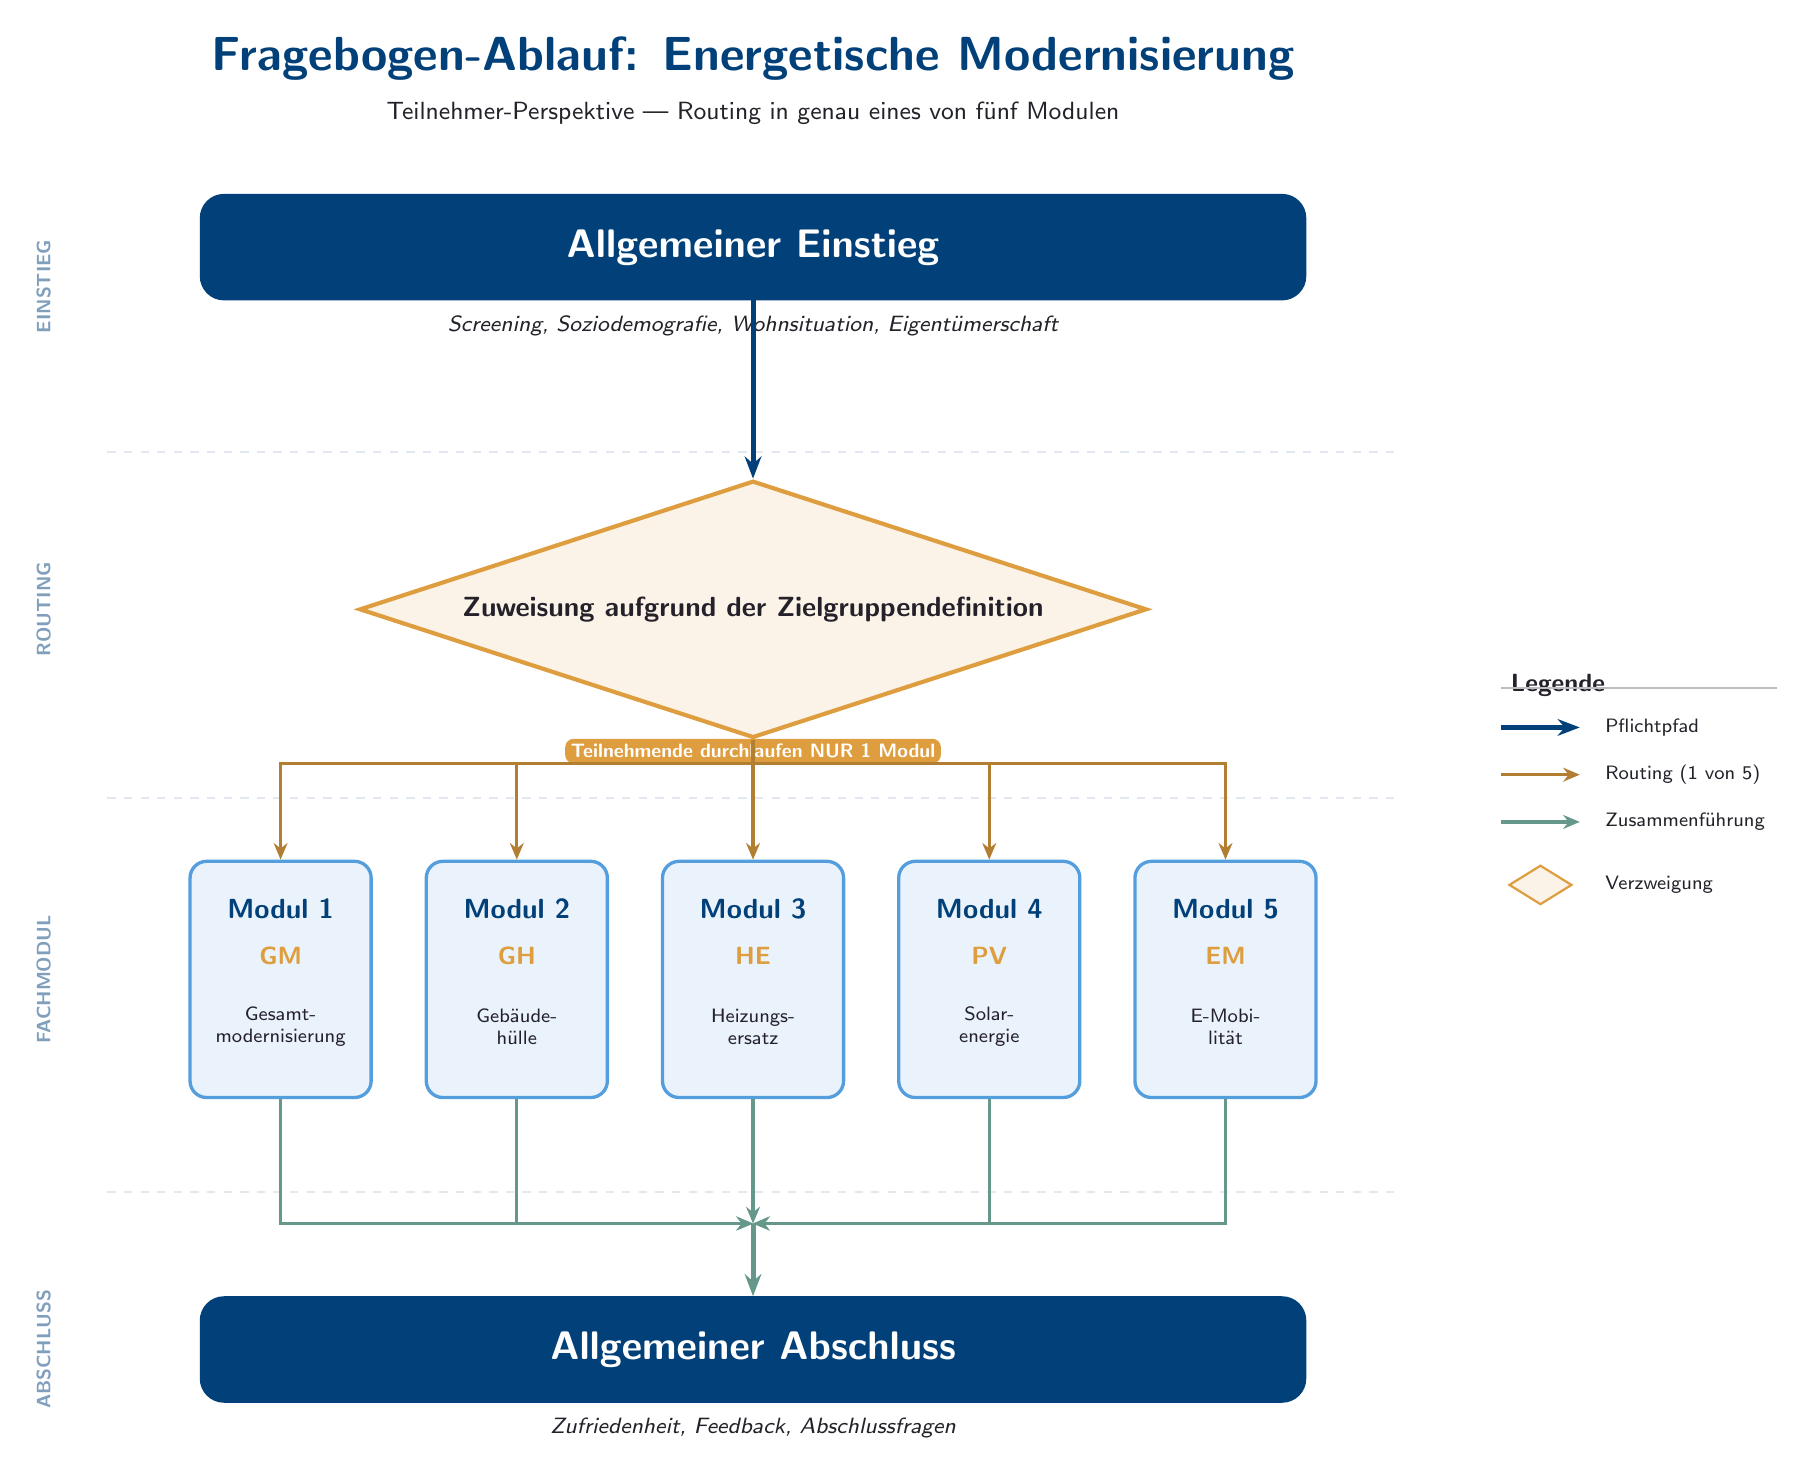
\begin{tikzpicture}[
    % Node styles
    startend/.style={
        rectangle, rounded corners=8pt,
        minimum width=14cm, minimum height=1.3cm,
        draw=fadarkblue, line width=1.5pt,
        fill=fadarkblue, text=white,
        font=\Large\bfseries\sffamily,
        align=center
    },
    modulbox/.style={
        rectangle, rounded corners=6pt,
        minimum width=2.3cm, minimum height=3cm,
        draw=falightblue, line width=1.2pt,
        fill=falightblue!12,
        align=center, inner sep=5pt
    },
    router/.style={
        diamond, aspect=2.8,
        minimum width=10cm, minimum height=1.8cm,
        draw=faorange, line width=1.5pt,
        fill=faorange!12,
        font=\normalsize\bfseries\sffamily,
        align=center, text=fadarkgray
    },
    arrow/.style={
        -{Stealth[length=8pt, width=6pt]},
        line width=1.8pt, color=fadarkblue
    },
    arrowroute/.style={
        -{Stealth[length=6pt, width=5pt]},
        line width=1.2pt, color=faorange!80!black
    },
    arrowmerge/.style={
        -{Stealth[length=6pt, width=5pt]},
        line width=1.2pt, color=famint!80!black
    },
    note/.style={
        font=\footnotesize\sffamily\itshape, text=fadarkgray
    },
    phaselabel/.style={
        font=\scriptsize\bfseries\sffamily, text=fadarkblue!50,
        rotate=90, anchor=south
    },
    badge/.style={
        font=\scriptsize\bfseries\sffamily,
        text=white, fill=faorange,
        rounded corners=3pt, inner sep=2pt
    }
]

% ===== TITLE =====
\node[font=\LARGE\bfseries\sffamily, text=fadarkblue] at (0, 3.2)
    {Fragebogen-Ablauf: Energetische Modernisierung};
\node[font=\small\sffamily, text=fadarkgray] at (0, 2.5)
    {Teilnehmer-Perspektive --- Routing in genau eines von f\"unf Modulen};

% ===== PHASE LABELS =====
\node[phaselabel] at (-8.8, 0.3) {EINSTIEG};
\node[phaselabel] at (-8.8, -3.8) {ROUTING};
\node[phaselabel] at (-8.8, -8.5) {FACHMODUL};
\node[phaselabel] at (-8.8, -13.2) {ABSCHLUSS};

% Phase separator lines
\draw[fadarkblue!12, line width=0.6pt, dashed] (-8.2, -1.8) -- (8.2, -1.8);
\draw[fadarkblue!12, line width=0.6pt, dashed] (-8.2, -6.2) -- (8.2, -6.2);
\draw[fadarkblue!12, line width=0.6pt, dashed] (-8.2, -11.2) -- (8.2, -11.2);

% ===== START =====
\node[startend] (start) at (0, 0.8) {Allgemeiner Einstieg};
\node[note] (startnote) at (0, -0.2) {Screening, Soziodemografie, Wohnsituation, Eigent\"umerschaft};

% ===== ROUTER =====
\node[router] (router) at (0, -3.8) {Zuweisung aufgrund der Zielgruppendefinition};

% Arrow Start -> Router
\draw[arrow] (start.south) -- (router.north);

% ===== NUR EINES badge =====
\node[badge] at (0, -5.6) {Teilnehmende durchlaufen NUR 1 Modul};

% ===== 5 MODULES =====
% Module 1
\node[modulbox] (m1) at (-6, -8.5) {};
\node[font=\normalsize\bfseries\sffamily, text=fadarkblue] at (-6, -7.6) {Modul 1};
\node[font=\small\bfseries\sffamily, text=faorange] at (-6, -8.2) {GM};
\node[font=\scriptsize\sffamily, text=fadarkgray, align=center] at (-6, -9.1) {Gesamt-\\modernisierung};

% Module 2
\node[modulbox] (m2) at (-3, -8.5) {};
\node[font=\normalsize\bfseries\sffamily, text=fadarkblue] at (-3, -7.6) {Modul 2};
\node[font=\small\bfseries\sffamily, text=faorange] at (-3, -8.2) {GH};
\node[font=\scriptsize\sffamily, text=fadarkgray, align=center] at (-3, -9.1) {Geb\"aude-\\h\"ulle};

% Module 3
\node[modulbox] (m3) at (0, -8.5) {};
\node[font=\normalsize\bfseries\sffamily, text=fadarkblue] at (0, -7.6) {Modul 3};
\node[font=\small\bfseries\sffamily, text=faorange] at (0, -8.2) {HE};
\node[font=\scriptsize\sffamily, text=fadarkgray, align=center] at (0, -9.1) {Heizungs-\\ersatz};

% Module 4
\node[modulbox] (m4) at (3, -8.5) {};
\node[font=\normalsize\bfseries\sffamily, text=fadarkblue] at (3, -7.6) {Modul 4};
\node[font=\small\bfseries\sffamily, text=faorange] at (3, -8.2) {PV};
\node[font=\scriptsize\sffamily, text=fadarkgray, align=center] at (3, -9.1) {Solar-\\energie};

% Module 5
\node[modulbox] (m5) at (6, -8.5) {};
\node[font=\normalsize\bfseries\sffamily, text=fadarkblue] at (6, -7.6) {Modul 5};
\node[font=\small\bfseries\sffamily, text=faorange] at (6, -8.2) {EM};
\node[font=\scriptsize\sffamily, text=fadarkgray, align=center] at (6, -9.1) {E-Mobi-\\lit\"at};

% ===== ARROWS: Router -> Modules =====
\coordinate (routeout) at ($(router.south) + (0, -0.3)$);
\draw[arrowroute] (router.south) -- (routeout) -| (m1.north);
\draw[arrowroute] (router.south) -- (routeout) -| (m2.north);
\draw[arrowroute] (router.south) -- (routeout) -| (m3.north);
\draw[arrowroute] (router.south) -- (routeout) -| (m4.north);
\draw[arrowroute] (router.south) -- (routeout) -| (m5.north);

% ===== END =====
\node[startend] (endbox) at (0, -13.2) {Allgemeiner Abschluss};
\node[note] at (0, -14.2) {Zufriedenheit, Feedback, Abschlussfragen};

% ===== ARROWS: Modules -> End =====
\coordinate (mergepoint) at (0, -11.6);
\draw[arrowmerge] (m1.south) |- (mergepoint);
\draw[arrowmerge] (m2.south) |- (mergepoint);
\draw[arrowmerge] (m3.south) -- (mergepoint);
\draw[arrowmerge] (m4.south) |- (mergepoint);
\draw[arrowmerge] (m5.south) |- (mergepoint);
\draw[arrow, color=famint!80!black] (mergepoint) -- (endbox.north);

% ===== LEGEND =====
\begin{scope}[shift={(9.5, -5)}]
    \node[font=\small\bfseries\sffamily, text=fadarkgray, anchor=north west] at (0, 0.5) {Legende};
    \draw[fadarkgray!30, line width=0.5pt] (0, 0.2) -- (3.5, 0.2);

    \draw[arrow] (0, -0.3) -- ++(1, 0);
    \node[font=\scriptsize\sffamily, text=fadarkgray, anchor=west] at (1.2, -0.3) {Pflichtpfad};

    \draw[arrowroute] (0, -0.9) -- ++(1, 0);
    \node[font=\scriptsize\sffamily, text=fadarkgray, anchor=west] at (1.2, -0.9) {Routing (1 von 5)};

    \draw[arrowmerge] (0, -1.5) -- ++(1, 0);
    \node[font=\scriptsize\sffamily, text=fadarkgray, anchor=west] at (1.2, -1.5) {Zusammenf\"uhrung};

    \node[diamond, aspect=1.5, draw=faorange, line width=0.8pt,
          fill=faorange!12, minimum width=0.8cm, minimum height=0.5cm]
          at (0.5, -2.3) {};
    \node[font=\scriptsize\sffamily, text=fadarkgray, anchor=west] at (1.2, -2.3) {Verzweigung};
\end{scope}

\end{tikzpicture}
\end{document}
